\chapter[Memories of Prof.\ G. Ramachandran]{Memories of\\ Prof.\ G. Ramachandran}\label{chap21}

\Authorline{Dr.\ B. A. Kagali}

\authinfo{Professor of Physics (retd.), Bangalore University}

I had the pleasure and privilege of meeting Prof. G Ramachandran on several occasions. Unfortunately, I was neither a student of Prof.\ Ramachandran nor his collaborator and so I did not have a long-term association with him.


I first met him in the University of Mysore as an examiner for the students who had completed minor projects with him. I found him a very affable person who would put his students at ease throughout the examination. The students had done their projects on topics related to polarisation of radiation and particles- a topic that seems to be one of his favourites.

The next time I met him was when he came as a guest faculty at Bangalore University specially invited to deliver lectures on Quantum Electrodynamics. I found him an expert speaker with so much confidence in the subject. He was teaching purely by memory without using notes or books. It was an amazing experience. Of course, the lectures passed over the heads of most of the postgraduate students!

On another day, I had the occasion of visiting him at his residence in Jayanagar, Bangalore after he retired from his association with IIA. On that occasion, he expressed a keen interest in setting up a `Study Circle' in Bangalore near his residence, so that like-minded faculty and students could meet once a week to deliberate on interesting topics and then develop collaborations to work on research problems. He had asked me to look for a convenient venue near his residence so that he could walk up to it without depending on others. However, for various reasons, such a study circle did not come up in time. I found him to be a person with a deep academic inclination and eagerness. He would often discuss new topics without having any reservations about his own status and reputation.

Another time I met Prof.\ Ramachandran was during the occasion when he was invited to deliver talks on Angular Momentum theory at K L E's Nijalingappa College in Bangalore. His lectures were well attended by students from all levels and as usual, I found him lecturing with ease and confidence on the classical and quantum notions associated with the angular. His talks were published later in the form of a book, I think.

On the whole, I found with my brief interactions with him spread over two or three decades, Prof.\ Ramachandran was a man of proverbial simple living and high thinking with a total dedication to the subject of his choice. He was quite friendly with students and collaborators. It is indeed very rare to find such individuals in the society.
\bigskip

\centerline{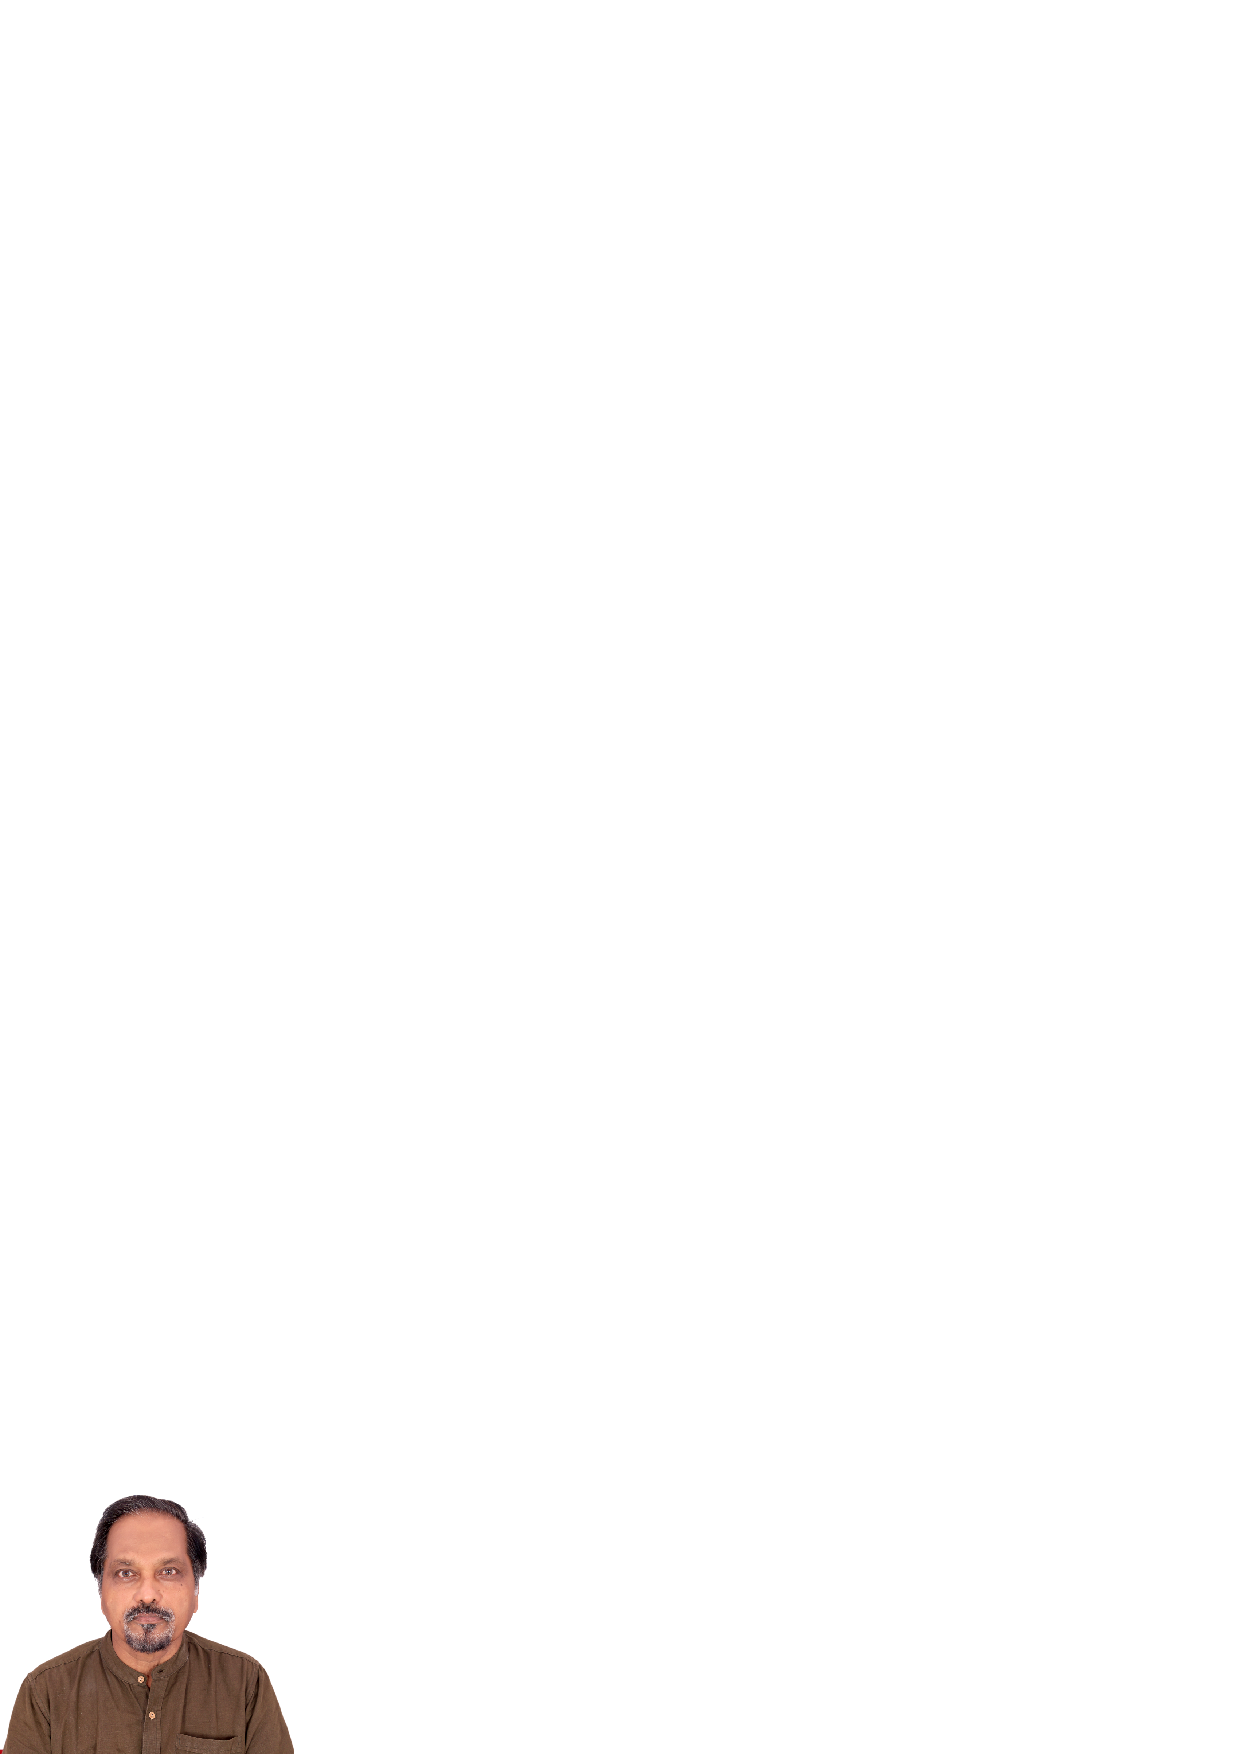
\includegraphics[scale=.6]{authorsphotos/Prof_B_A_Kagali.jpg}}
\smallskip

\authbio{B. A. Kagali}
\bigskip

\noindent
\textbf{Dr.\ B. A. Kagali} received MS from Purdue University in 1976, and Ph.D. from University of Texas at Austin, USA, in 1980. He joined the Physics Department, Gulbarga University, in 1981 and then moved over to the Department of Physics, Bangalore University, in 1986. He retired as a Professor in 2013. Currently he resides at Rajarajeshwarinagar, Bengaluru.
